% Options for packages loaded elsewhere
\PassOptionsToPackage{unicode}{hyperref}
\PassOptionsToPackage{hyphens}{url}
\PassOptionsToPackage{dvipsnames,svgnames,x11names}{xcolor}
%
\documentclass[
]{article}

\usepackage{amsmath,amssymb}
\usepackage{iftex}
\ifPDFTeX
  \usepackage[T1]{fontenc}
  \usepackage[utf8]{inputenc}
  \usepackage{textcomp} % provide euro and other symbols
\else % if luatex or xetex
  \usepackage{unicode-math}
  \defaultfontfeatures{Scale=MatchLowercase}
  \defaultfontfeatures[\rmfamily]{Ligatures=TeX,Scale=1}
\fi
\usepackage{lmodern}
\ifPDFTeX\else  
    % xetex/luatex font selection
\fi
% Use upquote if available, for straight quotes in verbatim environments
\IfFileExists{upquote.sty}{\usepackage{upquote}}{}
\IfFileExists{microtype.sty}{% use microtype if available
  \usepackage[]{microtype}
  \UseMicrotypeSet[protrusion]{basicmath} % disable protrusion for tt fonts
}{}
\usepackage{xcolor}
\usepackage[top=10pc,bottom=10pc,left=11pc,right=11pc,heightrounded]{geometry}
\setlength{\emergencystretch}{3em} % prevent overfull lines
\setcounter{secnumdepth}{-\maxdimen} % remove section numbering


\providecommand{\tightlist}{%
  \setlength{\itemsep}{0pt}\setlength{\parskip}{0pt}}\usepackage{longtable,booktabs,array}
\usepackage{calc} % for calculating minipage widths
% Correct order of tables after \paragraph or \subparagraph
\usepackage{etoolbox}
\makeatletter
\patchcmd\longtable{\par}{\if@noskipsec\mbox{}\fi\par}{}{}
\makeatother
% Allow footnotes in longtable head/foot
\IfFileExists{footnotehyper.sty}{\usepackage{footnotehyper}}{\usepackage{footnote}}
\makesavenoteenv{longtable}
\usepackage{graphicx}
\makeatletter
\def\maxwidth{\ifdim\Gin@nat@width>\linewidth\linewidth\else\Gin@nat@width\fi}
\def\maxheight{\ifdim\Gin@nat@height>\textheight\textheight\else\Gin@nat@height\fi}
\makeatother
% Scale images if necessary, so that they will not overflow the page
% margins by default, and it is still possible to overwrite the defaults
% using explicit options in \includegraphics[width, height, ...]{}
\setkeys{Gin}{width=\maxwidth,height=\maxheight,keepaspectratio}
% Set default figure placement to htbp
\makeatletter
\def\fps@figure{htbp}
\makeatother

% -----------------------
% CUSTOM PREAMBLE STUFF
% -----------------------

% -----------------
% Typography tweaks
% -----------------
% Indent size
\setlength{\parindent}{1pc}  % 1p0

% Fix widows and orphans
\usepackage[all,defaultlines=2]{nowidow}

% List things
\usepackage{enumitem}
% Same document-level indentation for ordered and ordered lists
\setlist[1]{labelindent=\parindent}
\setlist[itemize]{leftmargin=*}
\setlist[enumerate]{leftmargin=*}

% Wrap definition list terms
% https://tex.stackexchange.com/a/9763/11851
\setlist[description]{style=unboxed}


% For better TOCs
\usepackage{tocloft}

% Remove left margin in lists inside longtables
% https://tex.stackexchange.com/a/378190/11851
\AtBeginEnvironment{longtable}{\setlist[itemize]{nosep, wide=0pt, leftmargin=*, before=\vspace*{-\baselineskip}, after=\vspace*{-\baselineskip}}}


% -----------------
% Title block stuff
% -----------------

% Abstract
\usepackage[overload]{textcase}
\usepackage[runin]{abstract}
\renewcommand{\abstractnamefont}{\sffamily\footnotesize\bfseries\MakeUppercase}
\renewcommand{\abstracttextfont}{\sffamily\small}
\setlength{\absleftindent}{\parindent * 2}
\setlength{\absrightindent}{\parindent * 2}
\abslabeldelim{\quad}
\setlength{\abstitleskip}{-\parindent}


% Keywords
\newenvironment{keywords}
{\vskip -3em \hspace{\parindent}\small\sffamily{\sffamily\footnotesize\bfseries\MakeUppercase{Keywords}}\quad}
{\vskip 3em}

  
% Title
\usepackage{titling}
\setlength{\droptitle}{3em}
\pretitle{\par\vskip 5em \begin{flushleft}\LARGE\sffamily\bfseries}
\posttitle{\par\end{flushleft}\vskip 0.75em}


% Authors
%
% PHEW this is complicated for a number of reasons!
%
% When using \and with multiple authors, the article class in LaTeX wraps each 
% author block in a tabluar environment with a hardcoded center alignment. It's 
% possible to use \preauthor{} to start tabulars with a left alignment {l}, but 
% that only applies to the first author because the others all use \and with the 
% hardcoded {c}. But we can override the \and command and add our own {l}
%
% (See https://github.com/rstudio/rmarkdown/issues/1716#issuecomment-560601691 
% for an example of redefining \and to just be \\)
%
% That's all great, except tabulars have some amount of default horizontal 
% padding, which makes left-aligned author blocks not actuall get fully 
% left-aligned on the page. We can set the horizontal padding for the column to 
% 0, but it requires some wonky syntax: {@{\hspace{0em}}l@{}}
\renewcommand{\and}{\end{tabular} \hskip 3em \begin{tabular}[t]{@{\hspace{0em}}l@{}}}
\preauthor{\begin{flushleft}
           \lineskip 1.5em 
           \begin{tabular}[t]{@{\hspace{0em}}l@{}}}
\postauthor{\end{tabular}\par\end{flushleft}}

% Omit the date since the \published command does that
\predate{}
\postdate{}

% Command for a note at the top of the first page describing the publication
% status of the paper.
\newcommand{\published}[1]{%
   \gdef\puB{#1}}
   \newcommand{\puB}{}
   \renewcommand{\maketitlehooka}{%
       \par\noindent\footnotesize\sffamily \puB}


% ------------------
% Section headings
% ------------------
\usepackage{titlesec}
\titleformat*{\section}{\Large\sffamily\bfseries\raggedright}
\titleformat*{\subsection}{\large\sffamily\bfseries\raggedright}
\titleformat*{\subsubsection}{\normalsize\sffamily\bfseries\raggedright}
\titleformat*{\paragraph}{\small\sffamily\bfseries\raggedright}

% \titlespacing{<command>}{<left>}{<before-sep>}{<after-sep>}
% Starred version removes indentation in following paragraph
\titlespacing*{\section}{0em}{2em}{0.1em}
\titlespacing*{\subsection}{0em}{1.25em}{0.1em}
\titlespacing*{\subsubsection}{0em}{0.75em}{0em}


% -----------
% Footnotes
% -----------
% NB: footmisc has to come after biblatex because of conflicts
\usepackage[bottom, flushmargin]{footmisc}
\renewcommand*{\footnotelayout}{\footnotesize}

\addtolength{\skip\footins}{10pt}    % vertical space between rule and main text
\setlength{\footnotesep}{5pt}  % vertical space between footnotes


% ----------
% Captions
% ----------
\usepackage[font={small,sf}, labelfont={small,sf,bf}]{caption}


% --------
% Macros
% --------
% pandoc will not convert text within \begin{} XXX \end{} to Markdown and will
% treat it as regular TeX. Because of this, it's impossible to do stuff like
% this:

% \begin{landscape}
%
% | One | Two   |
% |-----+-------|
% | my  | table |
% | is  | nice  |
%
% \end{landscape}
%
% Since it'll render like: | One | Two | |—–+——-| | my | table | | is | nice |
% 
% BUT, from this http://stackoverflow.com/a/41945462/120898 we can get around
% this by creating new commands for \begin and \end, like this:
\newcommand{\blandscape}{\begin{landscape}}
\newcommand{\elandscape}{\end{landscape}}

% \blandscape
%
% | One | Two   |
% |-----+-------|
% | my  | table |
% | is  | nice  |
%
% \elandscape

% Same thing, but for generic groups
% But can't use \bgroup and \egroup because those are built-in TeX things
\newcommand{\stgroup}{\begingroup}
\newcommand{\fingroup}{\endgroup}


% ---------------------------
% END CUSTOM PREAMBLE STUFF
% ---------------------------
\usepackage{booktabs}
\usepackage{longtable}
\usepackage{array}
\usepackage{multirow}
\usepackage{wrapfig}
\usepackage{float}
\usepackage{colortbl}
\usepackage{pdflscape}
\usepackage{tabu}
\usepackage{threeparttable}
\usepackage{threeparttablex}
\usepackage[normalem]{ulem}
\usepackage{makecell}
\usepackage{xcolor}
\makeatletter
\@ifpackageloaded{caption}{}{\usepackage{caption}}
\AtBeginDocument{%
\ifdefined\contentsname
  \renewcommand*\contentsname{Table of contents}
\else
  \newcommand\contentsname{Table of contents}
\fi
\ifdefined\listfigurename
  \renewcommand*\listfigurename{List of Figures}
\else
  \newcommand\listfigurename{List of Figures}
\fi
\ifdefined\listtablename
  \renewcommand*\listtablename{List of Tables}
\else
  \newcommand\listtablename{List of Tables}
\fi
\ifdefined\figurename
  \renewcommand*\figurename{Figure}
\else
  \newcommand\figurename{Figure}
\fi
\ifdefined\tablename
  \renewcommand*\tablename{Table}
\else
  \newcommand\tablename{Table}
\fi
}
\@ifpackageloaded{float}{}{\usepackage{float}}
\floatstyle{ruled}
\@ifundefined{c@chapter}{\newfloat{codelisting}{h}{lop}}{\newfloat{codelisting}{h}{lop}[chapter]}
\floatname{codelisting}{Listing}
\newcommand*\listoflistings{\listof{codelisting}{List of Listings}}
\makeatother
\makeatletter
\makeatother
\makeatletter
\@ifpackageloaded{caption}{}{\usepackage{caption}}
\@ifpackageloaded{subcaption}{}{\usepackage{subcaption}}
\makeatother
\ifLuaTeX
  \usepackage{selnolig}  % disable illegal ligatures
\fi
\usepackage{bookmark}

\IfFileExists{xurl.sty}{\usepackage{xurl}}{} % add URL line breaks if available
\urlstyle{same} % disable monospaced font for URLs
\hypersetup{
  pdftitle={ARTS - methods},
  pdfauthor={Mirjam R. Rieger; Jan Schmitt; Paula Machin; Johann Musculus; Ralf Dittrich; Jannis Gottwald; Jonas Hoechst; Patrick Lampe},
  pdfkeywords={bird migration, radio-telemetry, stopover ecology},
  colorlinks=true,
  linkcolor={DarkSlateBlue},
  filecolor={Maroon},
  citecolor={DarkSlateBlue},
  urlcolor={DarkSlateBlue},
  pdfcreator={LaTeX via pandoc}}

% -----------------------
% END-OF-PREAMBLE STUFF
% -----------------------


% ----------
% BibLaTeX
% ----------
\usepackage[style=apa,backend=biber]{biblatex}

\setlength\bibitemsep{0pt}  % No space between bib entries
\renewcommand*{\bibfont}{\footnotesize}  % Use smaller font
\setlength\bibhang{\parindent}  % Match document indentation

% Fix biblatex's odd preference for using In: by default.
\renewbibmacro{in:}{%
  \ifentrytype{article}{}{%
  \printtext{\bibstring{}\intitlepunct}}}

\addbibresource{references.bib}

% ---------------------- 
% Title block elements
% ---------------------- 
\usepackage{orcidlink}  % Create automatic ORCID icons/links

\title{ARTS - methods}


\author{
{\large Mirjam R. Rieger~\orcidlink{0000-0002-7404-6023}}%
\thanks{Corresponding author.} \\%
University of Applied Science \\Eberhard Karls University \\%
{\footnotesize \url{mrieger@posteo.de}} \and
{\large Jan Schmitt~\orcidlink{xx}}%
 \\%
Eberhard Karls University \\%
{\footnotesize \url{xx}} \and
{\large Paula Machin~\orcidlink{xx}}%
 \\%
Eurofins MITOX group \\%
{\footnotesize \url{xx}} \and
{\large Johann Musculus~\orcidlink{xx}}%
 \\%
Eurofins MITOX group \\%
{\footnotesize \url{xx}} \and
{\large Ralf Dittrich~\orcidlink{xx}}%
 \\%
Eurofins MITOX group \\%
{\footnotesize \url{xx}} \and
{\large Jannis Gottwald~\orcidlink{xx}}%
 \\%
tRackIT systems \\%
{\footnotesize \url{gottwald@trackit.systems}} \and
{\large Jonas Hoechst~\orcidlink{0000-0002-7326-2250}}%
 \\%
tRackIT systems \\%
{\footnotesize \url{hoechst@trackit.systems}} \and
{\large Patrick Lampe~\orcidlink{xx}}%
 \\%
tRackIT systems \\%
{\footnotesize \url{lampe@trackit.systems}} \and
}

\date{}


% Typeset URLs in the same font as their parent environment
%
% This has to come at the end of the preamble, after any biblatex stuff because 
% some biblatex styles (like APA) define their own \urlstyle{}
\usepackage{url}
\urlstyle{same}

% ---------------------------
% END END-OF-PREAMBLE STUFF
% ---------------------------
\begin{document}
% ---------------
% TITLE SECTION
% ---------------
\published{\textbf{Thursday, June 13, 2024} \qquad working
manuscript \\ {\scriptsize Access the code, data, and analysis at
\url{https://github.com/m-rieger/MaisLE_ARTS.git}}}

\maketitle

\begin{abstract}
Abstract goes here.
\end{abstract}
\vskip 3em

\begin{keywords}
\def\sep{;\ }
bird migration\sep radio-telemetry\sep 
stopover ecology
\end{keywords}

% -------------------
% END TITLE SECTION
% -------------------


\section*{About}\label{about}
\addcontentsline{toc}{section}{About}

Paper to compare different methods for position estimation using
directional stations (quadrologgers) and omnidiretional stations
(monologgers), mainly based on data from maisC but supplemented with
data from maisD and melons (only quadrologgers).

We aim to publish it in Methods of Ecology and Evolution
\url{https://besjournals.onlinelibrary.wiley.com/journal/2041210x}

\section*{Abstract}\label{abstract}
\addcontentsline{toc}{section}{Abstract}

\section{Introduction}\label{introduction}

\section{Methods}\label{methods}

\subsection{stations}\label{stations}

\subsubsection{quadrologgers}\label{quadrologgers}

A station with 4 directional antennas, usually facing north, east,
south, and west. Antennas used were \textbf{Yagi} antennas (decribe
model and type, e.g.~refer to already existing paper with same setup)\\
\emph{--\textgreater{} show picture of antenna beams (by Ralf)}

\subsubsection{monologgers}\label{monologgers}

A station with 1 omnidirectional antenna facing upwards. Antennas used
were \textbf{????} antennas (describe model and type, e.g.~refer to
already existing paper with same setup)\\
\emph{--\textgreater{} show picture of antenna beam (tRackIT??)}

\subsection{tags}\label{tags}

\emph{--\textgreater{} describe different types of testtags (for maisC
and D same models, melons has different ones)}

\subsection{sample sites}\label{sample-sites}

\emph{--\textgreater{} maybe make a table to compare the different sites
with columns no. of quadrologgers, no. of monologgers, no. and type of
testtags, no. of testtracks, no. of circle tracks, no. of grid points
(and distance between them), site description (e.g.~difference in
elevation, vegetation, \ldots)}

\begin{longtable}[]{@{}
  >{\raggedright\arraybackslash}p{(\columnwidth - 20\tabcolsep) * \real{0.0461}}
  >{\raggedright\arraybackslash}p{(\columnwidth - 20\tabcolsep) * \real{0.2171}}
  >{\raggedright\arraybackslash}p{(\columnwidth - 20\tabcolsep) * \real{0.0724}}
  >{\raggedright\arraybackslash}p{(\columnwidth - 20\tabcolsep) * \real{0.3421}}
  >{\raggedright\arraybackslash}p{(\columnwidth - 20\tabcolsep) * \real{0.0329}}
  >{\raggedleft\arraybackslash}p{(\columnwidth - 20\tabcolsep) * \real{0.0461}}
  >{\raggedleft\arraybackslash}p{(\columnwidth - 20\tabcolsep) * \real{0.0329}}
  >{\raggedleft\arraybackslash}p{(\columnwidth - 20\tabcolsep) * \real{0.0592}}
  >{\raggedright\arraybackslash}p{(\columnwidth - 20\tabcolsep) * \real{0.0724}}
  >{\raggedleft\arraybackslash}p{(\columnwidth - 20\tabcolsep) * \real{0.0461}}
  >{\raggedright\arraybackslash}p{(\columnwidth - 20\tabcolsep) * \real{0.0329}}@{}}
\toprule\noalign{}
\begin{minipage}[b]{\linewidth}\raggedright
site
\end{minipage} & \begin{minipage}[b]{\linewidth}\raggedright
location
\end{minipage} & \begin{minipage}[b]{\linewidth}\raggedright
elevation
\end{minipage} & \begin{minipage}[b]{\linewidth}\raggedright
vegetation
\end{minipage} & \begin{minipage}[b]{\linewidth}\raggedright
area
\end{minipage} & \begin{minipage}[b]{\linewidth}\raggedleft
quadro
\end{minipage} & \begin{minipage}[b]{\linewidth}\raggedleft
mono
\end{minipage} & \begin{minipage}[b]{\linewidth}\raggedleft
testtags
\end{minipage} & \begin{minipage}[b]{\linewidth}\raggedright
testtracks
\end{minipage} & \begin{minipage}[b]{\linewidth}\raggedleft
circle
\end{minipage} & \begin{minipage}[b]{\linewidth}\raggedright
grid
\end{minipage} \\
\midrule\noalign{}
\endhead
\bottomrule\noalign{}
\endlastfoot
maisC & Vierlinden, Brandenburg, Germany & 5-7m asl & agriculture, tree
lines, ditches with reed & NA & 10 & 10 & 4 & NA & 8 & NA \\
maisD & Döbberin, Brandenburg, Germany & 47-59m asl & agriculture, tree
lines, lakes with reed and shrubs & NA & 8 & 0 & 3 & NA & 8 & NA \\
melons & NA & NA & NA & NA & NA & 0 & NA & NA & NA & NA \\
\end{longtable}

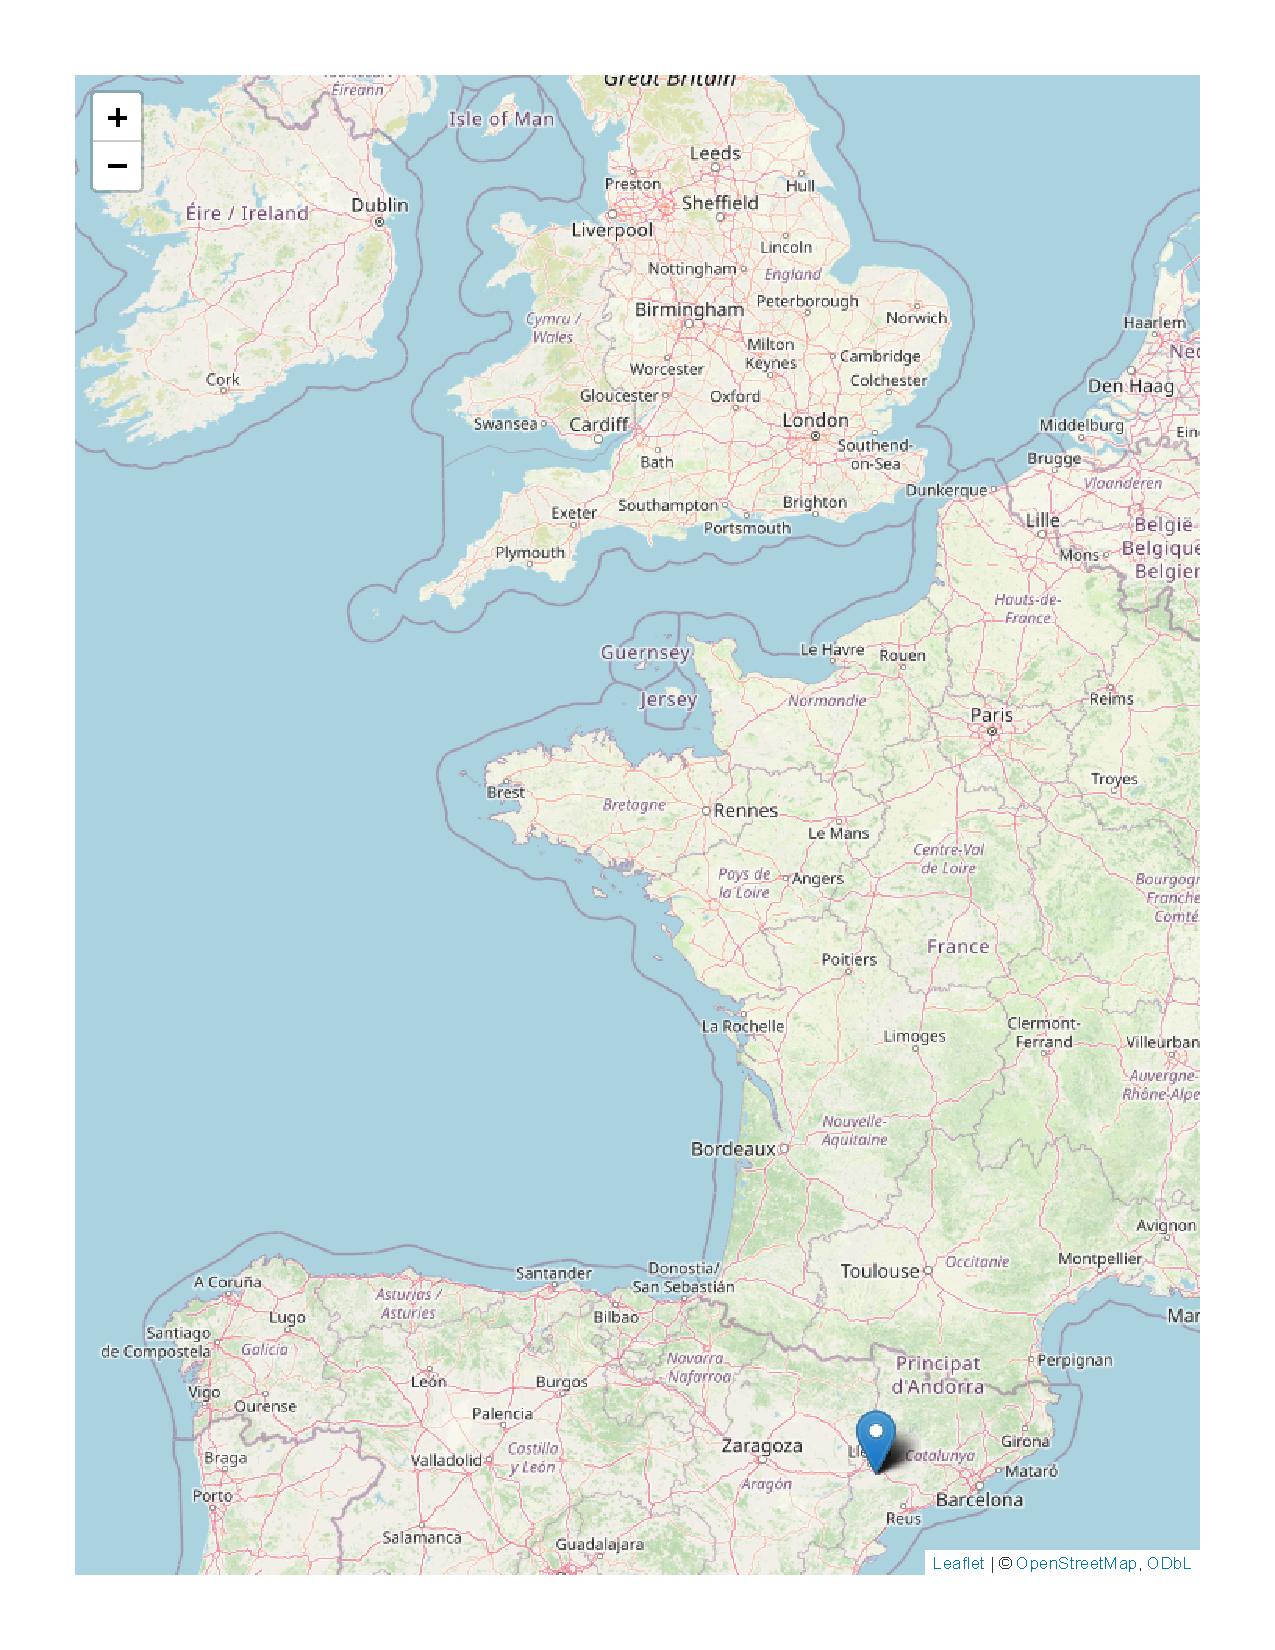
\includegraphics{MaisLE_ARTS_files/figure-pdf/figsite-1.pdf}

\subsubsection{maisC}\label{maisc}

\begin{itemize}
\tightlist
\item
  \textbf{10 quadrologgers} (maybe only 7 will be used due to twisted
  stations)\\
\item
  \textbf{10 monologgers} (maybe only 7 corresponding stations will be
  used)
\end{itemize}

3-4 testtags at different heights (0.5m, 1m, 1.5m, 2m)

\begin{itemize}
\tightlist
\item
  \textbf{XX testtracks}\\
\item
  \textbf{circle tracks} for stations c1l1-c6l1 (50m, 100m, 150m)\\
\item
  \textbf{gridpoints} with 100m distance to each other within a 300m (or
  400m???) radius around all stations
\end{itemize}

\subsubsection{maisD}\label{maisd}

\begin{itemize}
\tightlist
\item
  \textbf{8 quadrologgers}
\end{itemize}

3 testtags at different heights (0.5m, 1m, 1.5m)

\begin{itemize}
\tightlist
\item
  \textbf{XX testtracks}\\
\item
  \textbf{circle tracks} for all stations (50m, 100m, 150m)\\
\item
  \textbf{gridpoints} with 100m distance to each other within a 300m (or
  400m???) radius around all stations
\end{itemize}

\subsubsection{melons}\label{melons}

\begin{itemize}
\tightlist
\item
  \textbf{xx quadrologgers} (ask Paula)
\end{itemize}

xx testtags at different heights (???)

\begin{itemize}
\tightlist
\item
  \textbf{XX testtracks}\\
\item
  \textbf{circle tracks} for xx stations (50m, 100m, 150m)\\
\item
  \textbf{gridpoints} with ???m distance to each other within a 300m (or
  400m???) radius around all stations
\end{itemize}

\subsection{preparation of data}\label{preparation-of-data}

\emph{--\textgreater{} explain filtering process done by tRackIT}

\subsection{position estimation}\label{position-estimation}

We used xx different approaches for positions estimations, namely

\begin{itemize}
\tightlist
\item
  \textbf{bearings and triangulations}, e.g.~method xx and method xy\\
\item
  \textbf{antenna beams} for quadrologgers\\
\item
  \textbf{multilateration} (e.g.~another name) for monologgers\\
\item
  \textbf{mix of both}\\
\item
  \ldots{}
\end{itemize}

\emph{--\textgreater{} make a table as overview (e.g.~which method is
used for which type of station, \ldots)}

\subsection{comparison of methods}\label{comparison-of-methods}

\subsubsection{bearing accuracy}\label{bearing-accuracy}

For bearing and triangulation methods only. Uses deviance between true
angle (based on GPS position) and estimated angle. Should be accumulated
around 0. If it is constantly shifted to the left or right, this might
be an indicator that the antenna itself was shifted by some degrees.
This might be used as a correction factor (also for other approaches) to
redefine the northern orientation. If it shifts over time, one might
either consider using different correction factors for the northern
orientation over time or to exclude the station

\subsubsection{position accuracy}\label{position-accuracy}

For all methods.

\section{Results}\label{results}

\section{Discussion}\label{discussion}


\printbibliography[title=References]


\end{document}
